\documentclass[10pt,a4paper]{article}
\usepackage[T1]{fontenc}
\usepackage[a4paper,left=2cm,right=2cm,top=2.1cm,bottom=2.2cm,headsep=0.45cm]{geometry}
\usepackage{amsmath,amssymb}
\usepackage{graphicx}
\usepackage{booktabs,tabularx,multirow}
\usepackage{caption}
\captionsetup{font=small,skip=3pt}
\usepackage[dvipsnames]{xcolor}
\usepackage[most]{tcolorbox}
\usepackage{titlesec}
\usepackage{fancyhdr}
\usepackage{eso-pic}
\usepackage{enumitem}
\usepackage{tikz}
\usetikzlibrary{positioning,arrows.meta,fit}
\usepackage[colorlinks=true,linkcolor=linkpink,urlcolor=linkpink,citecolor=linkpink]{hyperref}

\definecolor{accent}{RGB}{194,24,91}
\definecolor{linkpink}{RGB}{233,30,140}
\definecolor{boxpink}{RGB}{252,230,238}

% IIT Madras watermark on every page
\AddToShipoutPictureBG{\AtPageCenter{\makebox(0,0){\tikz\node[opacity=0.11]{
\includegraphics[width=8.5cm]{iitm_logo.png}};}}}

% header and footer
\pagestyle{fancy}
\fancyhf{}
\fancyhead[L]{\footnotesize\bfseries Madhav (CS23B035), Nitin (EE23B141)}
\fancyhead[R]{\footnotesize\bfseries CS6886 Course Project}
\fancyfoot[C]{\thepage}
\renewcommand{\headrulewidth}{0.4pt}
\fancypagestyle{plain}{\fancyhf{}\fancyfoot[C]{\thepage}\renewcommand{\headrulewidth}{0pt}}

% section titles
\titleformat{\section}{\Large\sffamily\bfseries}{\textcolor{accent}{\S\thesection}}{0.5em}{}
\titleformat{\subsection}{\large\sffamily\bfseries}{\textcolor{accent}{\S\thesubsection}}{0.5em}{}
\titlespacing*{\section}{0pt}{10pt}{6pt}
\titlespacing*{\subsection}{0pt}{8pt}{4pt}

% content box
\newtcolorbox{content}{enhanced,breakable,colback=boxpink,frame hidden,arc=3mm,boxrule=0pt,
  left=4mm,right=4mm,top=3mm,bottom=3mm,before skip=2pt,after skip=4pt,
  before upper={\setlength{\parskip}{8pt}}}

\setlength{\parindent}{0pt}
\setlength{\parskip}{5pt}
\linespread{1.18}\selectfont
\setlist{itemsep=2pt,topsep=2pt}

\begin{document}
\thispagestyle{plain}

\begin{center}
  {\LARGE\sffamily\bfseries CS6886 Course Project}\\[8pt]
  {\large\scshape Madhav (CS23B035) \quad Nitin (EE23B141)}
\end{center}

\section{Introduction to the Problem}
\begin{content}
Spiking neural networks (SNNs) are often called far more energy-efficient than normal networks, because they
replace multiplies with additions triggered by sparse spikes. Most SNN accelerators use rate coding, where a value
$q$ is sent as $q$ spikes, so a 4-bit activation can cost up to 15 spikes. Time-to-first-spike (TTFS) coding
sends a single spike and lets its time carry the value. A quantised network (QNN) with $n$-bit activations
converts exactly into a TTFS network with $T = 2^n - 1$ ticks.

The question is whether this actually saves energy in hardware once memory, control and clocking are counted, and
against baselines that are just as optimised. We build a TTFS accelerator tile, TTFS-64, and compare it with
SparTen, APEX and Eyeriss using measured power. We then ask where the gain comes from, and which spike code
should carry the signed activations of language models.

\textbf{GitHub repository:} \href{https://github.com/Madhav1729/TTFS}{Repository Link}
\quad \textbf{Checkpoints:} \href{https://drive.google.com/file/d/1ULRXTGxmAl8MLo_yqgPOb0wExdkZ89UQ/view?usp=sharing}{Drive Link}
\end{content}

\section{Prior Work and Baselines}
\begin{content}
SparTen~\cite{sparten} is a sparse CNN accelerator that multiplies only non-zero weight and activation pairs,
using bitmask matching in 32 units. It is our sparse QNN baseline at W4A4. LoAS~\cite{loas} and APEX~\cite{apex}
are accelerators for rate-coded SNNs; we use APEX with 16 INT4 processing elements at $T = 15$. Eyeriss~\cite{eyeriss}
is the dense reference. Otters~\cite{otters} turns BERT~\cite{bert} into a TTFS transformer with binary weights
and 4-bit activations, which we use for the language workload. Yan et al.~\cite{yan} argue on paper that SNN
energy savings shrink once memory is counted; we check this in RTL. The CNN is a W4A4 VGG-16~\cite{cifarmodels}
on CIFAR-100~\cite{cifar} (71.41\,\% accuracy).
\end{content}

\section{Idea and Implementation}
\subsection{Exact TTFS with S/U lanes}
\begin{content}
A TTFS neuron needs $U = \sum_i w_i\,(T - t_i)$, where $t_i$ is the tick at which input $i$ fired. If spikes
arrive in tick order, two registers are enough: on a spike $S \mathrel{+}= w$, and at the end of every tick
$U \mathrel{+}= S$. Each weight is then counted exactly $T - t_i$ times, with no multiplier. The neuron fires at
the first tick where $U$ crosses a threshold, which gives exactly the QNN output.
\end{content}

\newpage
\subsection{TTFS-64 architecture}
\begin{content}
\begin{center}
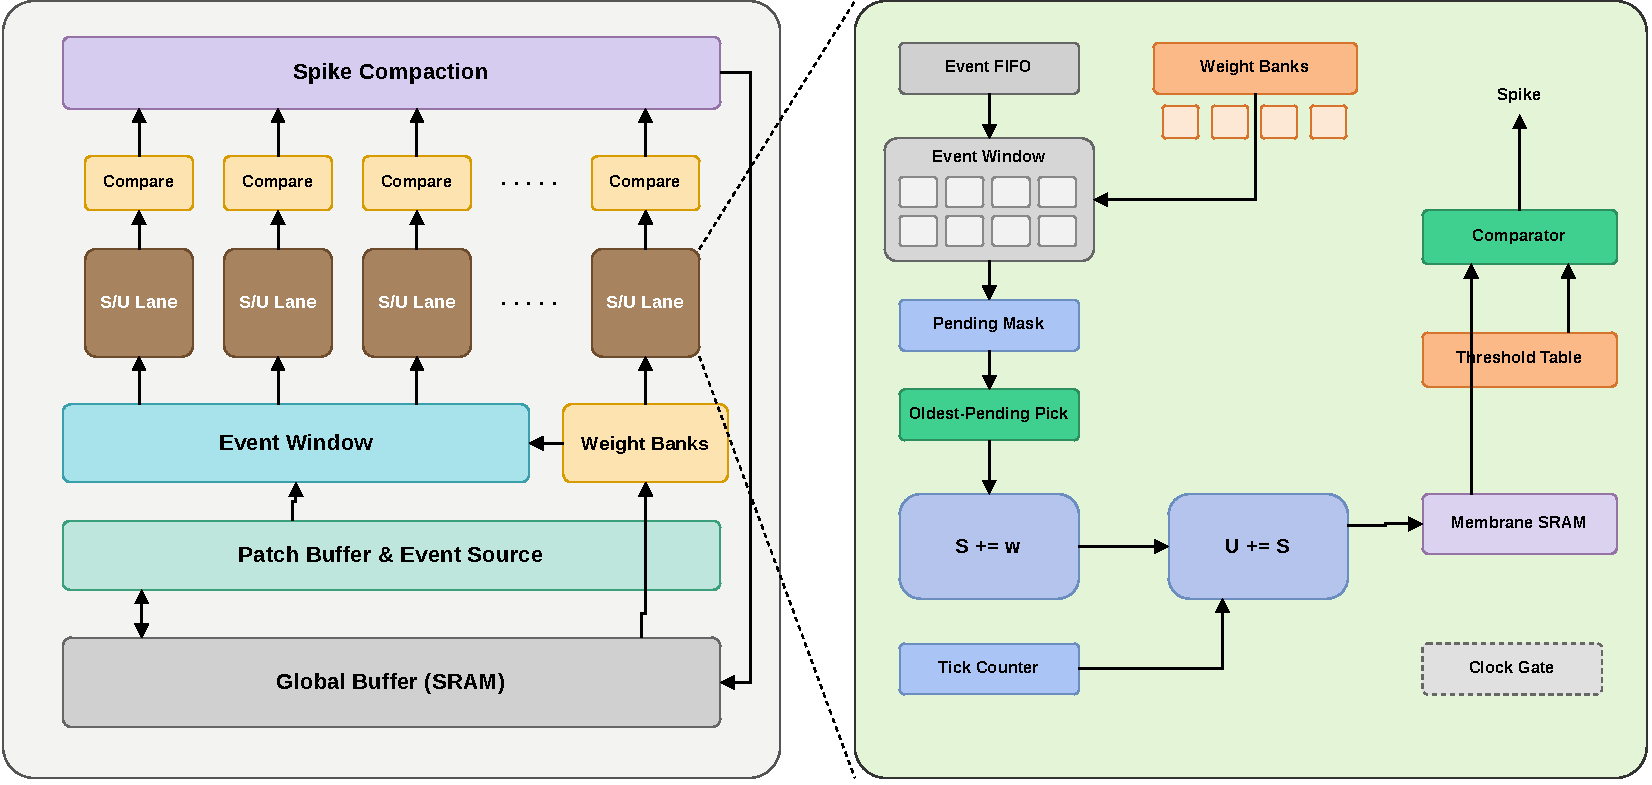
\includegraphics[width=\linewidth]{arch.pdf}
\captionof{figure}{TTFS-64 tile (left) and one S/U lane (right).}\label{fig:arch}
\end{center}
The tile computes 64 output channels at a time (Figure~\ref{fig:arch}). Inputs for a group of 32 pixels are
loaded once into a patch buffer, and the event source turns them into spikes sorted by tick. Spikes enter a
16-slot event window, and each slot fetches its weight column from four weight banks and sends it to all 64
lanes. Each lane only marks the slots where its own weight is non-zero, and adds the oldest one first, so idle
lanes never wait for zero weights.

Inside a lane, $S$ collects weights and $U$ adds $S$ at every tick; ticks with $S = 0$ are skipped. At the end
of a pass, $U$ is added into the membrane SRAM. When a group of pixels is done, each lane compares its membrane
against a shared threshold table, one tick at a time, and the spikes are compacted and written back. We also
added clock gating to each lane, so its registers switch only when something changes. This is exact and cuts
lane power by 11--13\,\%.
\end{content}

\subsection{Polarity TTFS for language models}
\begin{content}
Transformer activations are signed, but TTFS can only send non-negative values. The common fix adds an offset,
which turns the most common value, zero, into a spike. Instead we send $|q|$ as the spike time and the sign as one
extra bit, so zero stays silent. Only the magnitude is timed, so we need $T = 8$ ticks instead of 15. On the Otters
BERT, all 73 converted layers match the QNN output.
\end{content}

\subsection{Measurement flow}
\begin{content}
All designs are written in SystemVerilog and simulated in Verilator on all 12 conv layers of one image, with every
output checked bit-exactly. Power comes from Design Compiler (NanGate 45\,nm, 5\,ns) using switching activity
from the same simulations. All SRAMs are priced with CACTI~7~\cite{cacti} for every design alike, and TTFS and
SparTen share the same global buffer and weight encoding.
\end{content}

\section{Evaluation}
\subsection{CNN results}
\begin{content}
\begin{center}\small
\captionof{table}{Energy per image ($\mu$J), latency and area; gains relative to TTFS-64.}\label{tab:cnn}
\setlength{\tabcolsep}{4.5pt}
\begin{tabular}{llrrrrr}
\toprule
Sparsity & Design & Energy & Latency (ms) & Area (mm$^2$) & Energy gain & EDP gain \\
\midrule
\multirow{4}{*}{40\,\%} & TTFS-64 (ours) & \textbf{226.2} & \textbf{8.40} & \textbf{0.334} & -- & -- \\
 & SparTen W4/A4 & 396.4 & 12.15 & 0.584 & 1.75$\times$ & 2.54$\times$ \\
 & APEX ($T{=}15$) & 1421.1 & 38.37 & 0.567 & 6.28$\times$ & 28.7$\times$ \\
 & Eyeriss INT4 & 2326.8 & 35.32 & 1.778 & 10.3$\times$ & 43.3$\times$ \\
\midrule
\multirow{3}{*}{70\,\%} & TTFS-64 (ours) & \textbf{163.7} & \textbf{6.22} & & -- & -- \\
 & SparTen W4/A4 & 270.0 & 8.28 & & 1.65$\times$ & 2.19$\times$ \\
 & APEX & 1078.7 & 26.10 & & 6.59$\times$ & 27.6$\times$ \\
\midrule
\multirow{3}{*}{98\,\% (LoAS)} & TTFS-64 (ours) & \textbf{85.5} & \textbf{3.64} & & -- & -- \\
 & SparTen W4/A4 & 148.6 & 5.14 & & 1.74$\times$ & 2.45$\times$ \\
 & APEX & 646.5 & 12.16 & & 7.56$\times$ & 25.3$\times$ \\
\bottomrule
\end{tabular}
\end{center}
TTFS-64 uses 1.65--1.75$\times$ less energy than SparTen, is 1.33--1.45$\times$ faster and 1.75$\times$ smaller.
Against the rate-coded APEX the gain is 6.3--7.6$\times$, and Eyeriss, which cannot skip zeros, is 10--25$\times$
worse.
\end{content}

\subsection{Where the gain comes from}
\begin{content}
\begin{center}
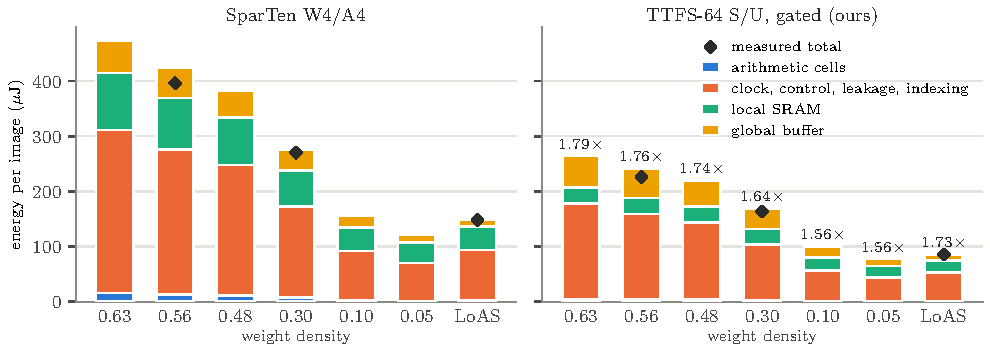
\includegraphics[width=\linewidth]{fig_sweep.pdf}
\captionof{figure}{Energy per image by cause across weight densities. Diamonds are measured totals.}\label{fig:sweep}
\end{center}
Across all weight densities the gain stays between 1.56 and 1.79$\times$ (Figure~\ref{fig:sweep}). Surprisingly,
only 2--5\,\% of the saving comes from replacing multiplies with adds. Most of it comes from the dataflow: one
weight column is shared by 64 small lanes, while SparTen needs matching logic and buffers in each of its 32 units.
Arithmetic is only 1--3\,\% of SparTen's energy, so even a free multiplier would barely help it.
\end{content}

\subsection{Roofline analysis}
\begin{content}
\begin{center}
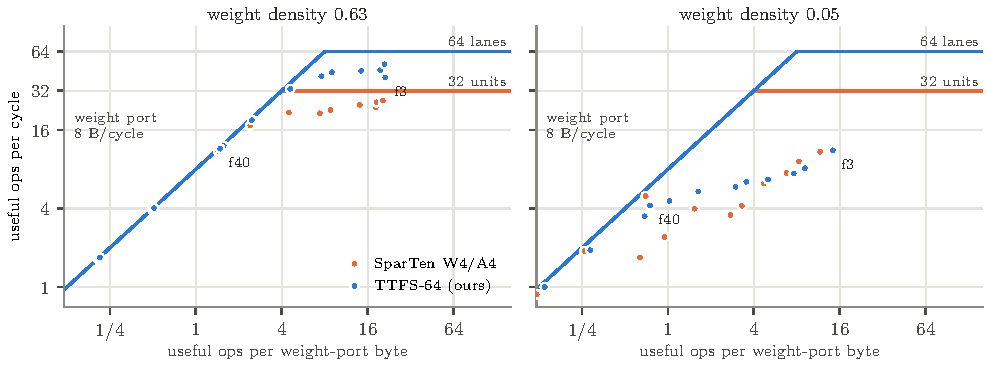
\includegraphics[width=\linewidth]{fig_roofline.pdf}
\captionof{figure}{Roofline of the 12 conv layers. Both designs share the same 8\,B/cycle weight port.}\label{fig:roof}
\end{center}
Figure~\ref{fig:roof} shows three regimes. Early layers reuse each weight across many pixels and are
compute-bound, so TTFS with 64 lanes runs 1.7--1.9$\times$ faster than SparTen with 32 units. Late layers have
few pixels, sit on the memory roof, and both designs run at the same speed. At very high sparsity every layer
falls below both roofs, because control overhead dominates.
\end{content}

\subsection{Language models}
\begin{content}
\begin{center}\small
\captionof{table}{Spike codes on one BERT-base encoder layer (128 tokens).}\label{tab:bert}
\begin{tabular}{lrrrr}
\toprule
Design & W1A4 ($\mu$J) & vs ours & W4A4 ($\mu$J) & vs ours \\
\midrule
Polarity TTFS, $T{=}8$ (ours) & \textbf{1852} & -- & \textbf{1393} & -- \\
Offset TTFS, $T{=}15$ & 2376 & 1.28$\times$ & 1782 & 1.28$\times$ \\
Bit-serial & 2204 & 1.19$\times$ & 1654 & 1.19$\times$ \\
Rate coding & 3432 & 1.85$\times$ & 2532 & 1.82$\times$ \\
SparTen W4/A4 & 3858 & 2.08$\times$ & 2746 & 1.97$\times$ \\
QNN with the same dataflow & 1852 & 1.00$\times$ & 1474 & 1.06$\times$ \\
\bottomrule
\end{tabular}
\end{center}
On a real BERT layer, polarity coding is 1.28$\times$ cheaper than offset TTFS, since about a quarter of the
inputs are zero and now stay silent. It also beats bit-serial and rate coding. However, a QNN with the same
dataflow is just as good (1.00--1.06$\times$), which again shows that the gain is in the dataflow.

For LLMs the picture is worse. Decoding reads every weight once per token, so it is memory-bound. For a 7B INT4
model, reading the weights costs about 111\,mJ per token while all the multiplies cost about 2\,mJ, so spiking
can save at most about 2\,\%.
\end{content}

\subsection{Conclusion}
\begin{content}
With measured power and fair memory pricing, a TTFS tile is 1.65--1.75$\times$ more efficient than a strong
sparse QNN accelerator and 6--8$\times$ more efficient than a rate-coded SNN accelerator, and polarity coding is
the best way to send signed activations. But the gain comes from the dataflow, not from the spike itself. The
biggest wins for spiking hardware are against rate coding. Our main limitations are split synthesis (wires
between blocks are not counted) and a single test image.
\end{content}

\newpage
{\Large\sffamily\bfseries References}
\renewcommand{\refname}{}
\vspace{-8mm}
\begin{thebibliography}{99}\setlength{\itemsep}{2pt}\small
\bibitem{sparten} A. Gondimalla, N. Chesnut, M. Thottethodi, T. N. Vijaykumar, ``SparTen: A Sparse Tensor
  Accelerator for Convolutional Neural Networks,'' MICRO 2019.
\bibitem{loas} R. Yin, Y. Kim, D. Wu, P. Panda, ``LoAS: Fully Temporal-Parallel Dataflow for Dual-Sparse
  Spiking Neural Networks,'' MICRO 2024.
\bibitem{apex} D. Bawa Venkatesh, S. Radhakrishnan, R. Rakshit, G. Srinivasan, ``APEX: A Dual-Sparsity
  Accelerator for Precise and Efficient SNN Inference,'' arXiv:2608.19046, 2026.
\bibitem{eyeriss} Y.-H. Chen, T. Krishna, J. Emer, V. Sze, ``Eyeriss: An Energy-Efficient Reconfigurable
  Accelerator for Deep Convolutional Neural Networks,'' IEEE JSSC, 2017.
\bibitem{otters} Z. Yan, J. Mao et al., ``Otters: An Energy-Efficient Spiking Transformer via Optical
  Time-to-First-Spike Encoding,'' ICLR 2026, \url{https://arxiv.org/abs/2509.18968}.
\bibitem{yan} Z. Yan, Z. Bai, K. Tang, W.-F. Wong, ``Reconsidering the Energy Efficiency of Spiking Neural
  Networks Inference from Analytical Perspectives,'' arXiv:2409.08290, \url{https://arxiv.org/abs/2409.08290}.
\bibitem{cacti} R. Balasubramonian, A. B. Kahng, N. Muralimanohar, A. Shafiee, V. Srinivas, ``CACTI 7: New
  Tools for Interconnect Exploration in Innovative Off-Chip Memories,'' ACM TACO, 2017.
\bibitem{cifarmodels} Y. Chen, Pretrained CIFAR-10/100 models in PyTorch,
  \url{https://github.com/chenyaofo/pytorch-cifar-models}.
\bibitem{cifar} A. Krizhevsky, ``Learning Multiple Layers of Features from Tiny Images,'' 2009.
\bibitem{bert} J. Devlin, M.-W. Chang, K. Lee, K. Toutanova, ``BERT: Pre-training of Deep Bidirectional
  Transformers for Language Understanding,'' NAACL 2019.
\bibitem{glue} A. Wang et al., ``GLUE: A Multi-Task Benchmark and Analysis Platform for Natural Language
  Understanding,'' ICLR 2019.
\bibitem{code} Project code: \url{https://github.com/Madhav1729/TTFS}; checkpoints:
  \url{https://drive.google.com/file/d/1ULRXTGxmAl8MLo_yqgPOb0wExdkZ89UQ/view?usp=sharing}.
\end{thebibliography}
\end{document}
